\section{Ejercicio 1: Tecnolog\'ias TTL, RTL, NMOS y CMOS}
Es de inter\'es estudiar los par\'ametros
que establecen los l\'imites f\'isicos al modelo conceptual de las compuertas l\'ogicas para diferentes tecnolog\'ias y topolog\'ias, dise\~nando con diferentes tecnolog\'ias 
una compuerta NOT y se asume que el lector tiene un conocimiento del funcionamiento de los dispositivos empleados en este estudio.

\subsection{An\'alisis te\'orico}
En los an\'alisis realizados para reproducir los circuitos ilustrados en la Fig. \ref{fig:circuitos}, se emplean transistores NPN $BC547$ con un $hFE_{min} = 110$, una $V_{CE_{SAT}} \approx 0.3V$. 
Luego para los MOSFET se emplea un par complementario $IRFZ44N$ y $IRF9530$. Se alimenta con $V_{CC} = V_{DD} = 5V$.

\begin{figure}[H]
    \centering
    \begin{tabular}{c c}
        \includegraphics[scale=0.35]{../EJ1/Recursos/rtl_circuit.png} &
        \includegraphics[scale=0.35]{../EJ1/Recursos/ttl_circuit.png} \\
        \includegraphics[scale=0.35]{../EJ1/Recursos/mos_circuit.png} &
        \includegraphics[scale=0.35]{../EJ1/Recursos/cmos_circuit.png} 
    \end{tabular} 
    \caption{Implementaci\'on en diversas tecnolog\'ias y topolog\'ias de Compuerta NOT}
    \label{fig:circuitos}
\end{figure}

\paragraph*{Tecnolog\'ia RTL:} Se opera un transistor $Q_1$ en conmutaci\'on con modos de saturaci\'on y corte, para ello se define arbitrariamente una resistencia $R_C = 10k\Omega$, se asume $Q_1$ en saturaci\'on y luego la corriente de colector
se establece como $I_{C_{SAT}} = \frac{V_{CC} - V_{CE_{SAT}}}{R_C} \approx 480 \mu A$, con lo cual con una resistencia de base $R_B = 470k\Omega$ se cumple la condici\'on de saturaci\'on.
\paragraph*{Tecnolog\'ia TTL:} Opera de igual forma que el caso RTL, en principio se asumen valores de resistencias iguales donde $R_1 = 470 k \Omega$ y $R_2 = 10k \Omega$. La diferencia principal es que la corriente de base del transistor de salida $Q_2$ es controlada por la de colector
del transistor de entrada $Q_1$, con lo cual los tiempos de recuperaci\'on se ven reducidos ya que se enciende y apaga con mucha m\'as corriente que antes, debiendose esperar menor tiempo de propagaci\'on o transici\'on.
\paragraph*{Tecnolog\'ia MOS:} Se opera un MOSFET de canal N en conmutaci\'on en modo de corte y lineal, para ello se garantiza que la resistencia $R_D$ sea lo suficientemente grande para no saturar el canal. Se propone una $R_D = 10k \Omega$. Se tiene en cuenta que el $V_{TH_{MAX}} = 4V < 5V$.
\paragraph*{Tecnolog\'ia CMOS:} Se evita usar una resistencia en el Drain usando redes de pull-up y pull-down con transistores MOS complementarios cuya $|V_{TH}| = 4V$.

\subsection{Niveles de tensi\'on}
La sintetizaci\'on de circuitos l\'ogicos implica la interconexi\'on de compuertas integradas que seg\'un su tecnolog\'ia y topolog\'ia maneja niveles de tensi\'on para los estados l\'ogicos que puede diferir con el resto, para esto
es de inter\'es analizar tales magnitudes en la implementaci\'on de los cuatro circuitos ilustrados previamente.

\subsubsection{Proceso de medici\'on}
Se genera una se\~nal de entrada triangular con una simetr\'ia del $50\%$ desde $0V$ hasta $5V$, con frecuencia a convenir menor a $f = 100Hz$. Luego, con un osciloscopio
se miden la entrada y la salida, utilizando puntas de prueba x10 con la menor capacidad par\'asita posible para no introducir transitorios superiores.
Finalmente, se descargan y procesan las mediciones, para localizar los puntos donde la derivada con $-1$. Adem\'as, se calculan los margenes de ruido como las 
diferencias correspondientes estados altos y bajos de entrada y salida.

\begin{figure}[H]
    \centering
    \begin{tabular}{c c}
        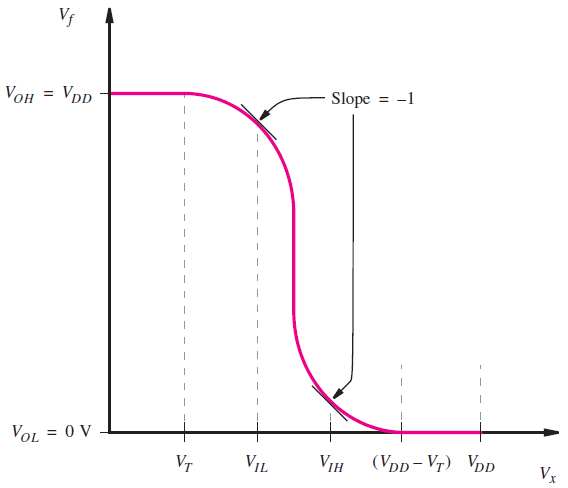
\includegraphics[scale=0.45]{../EJ1/Recursos/logic_leves.PNG} &
        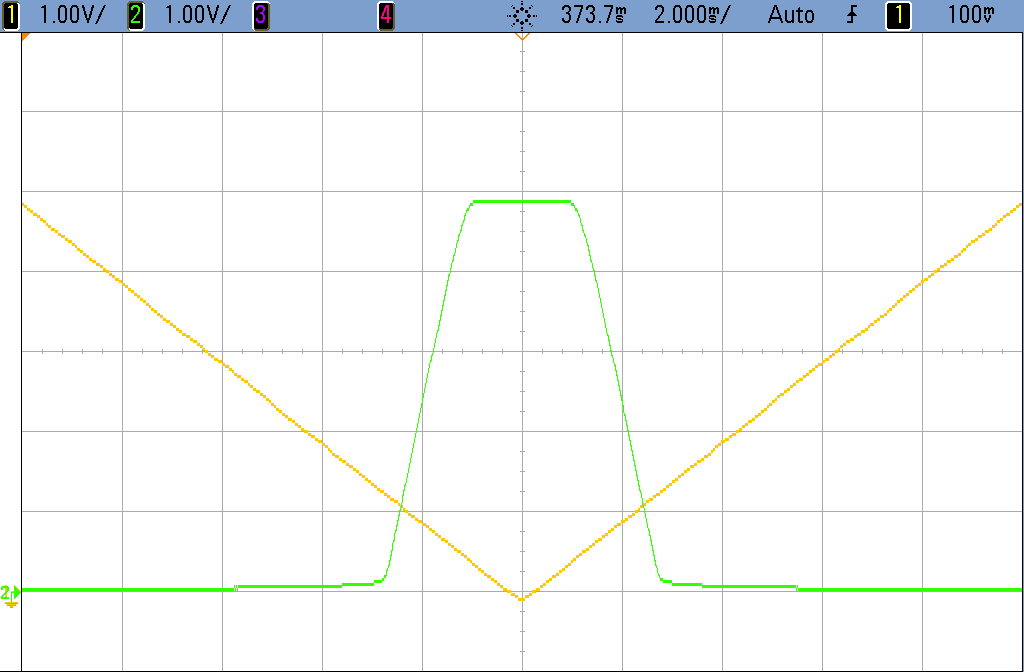
\includegraphics[scale=0.23]{../EJ1/Mediciones/Osciloscopio/Segundo_Intento/Voltage_Levels_RTL/cropped_scope_3.png}
    \end{tabular}
    \caption{$V_o(V_i)$ y medici\'on entrada(amarilla) y salida(verde).}
    \label{fig:logic_levels}
\end{figure}

\begin{table}[H]
    \centering
    \begin{tabular}{c c c c c c c}
        Circuito & VIH & VIL & VOH & VOL & NMH & NML \\
        \hline \\
        RTL & $1.33V$ & $0.28V$ & $4.89V$ & $0.11V$ & $3.55V$ & $0.16V$ \\
        TTL & $0.56V$ & $0.3V$ & $4.89V$ & $0.01V$ & $4.32V$ & $0.29V$ \\
        MOS & $2.7V$ & $1.94V$ & $4.89V$ & $0.04V$ & $2.19V$ & $1.89V$ \\
        CMOS & $2.89V$ & $1.7V$ & $4.94V$ & $0.04V$ & $2.04V$ & $1.66V$ \\
        \hline
    \end{tabular} 
    \caption{Resultados de los niveles de tensi\'on}
\end{table}

\begin{table}[H]
    \centering
    \begin{tabular}{c c c c c c c}
        Circuito & VIH & VIL & VOH & VOL & NMH & NML \\
        \hline \\
        RTL & $1.31V$ & $0.25V$ & $4.89V$ & $0.13V$ & $3.58V$ & $0.12V$ \\
        TTL & $0.55V$ & $0.31V$ & $4.89V$ & $0.01V$ & $4.33V$ & $0.29V$ \\
        MOS & $2.53V$ & $2.1V$ & $4.88V$ & $0.01V$ & $2.34V$ & $2.09V$ \\
        CMOS & $2.83V$ & $1.44V$ & $4.94V$ & $0.04V$ & $2.12V$ & $1.40V$ \\
        \hline
    \end{tabular} 
    \caption{Resultados de los niveles de tensi\'on con carga de $C = 1nF$}
    \label{table:voltage_levels_charged}
\end{table}

\subsubsection{An\'alisis de resultados}
De RTL a TTL disminuye el valor de VIH ya que, en TTL, se apaga el transistor de salida con la corriente de colector del primero. Por otro lado, es de esperar que los valores de VOH entre tales tecnolog\'ias no difieran,
dado que en presentan la misma malla de salida, no obstante se asume que la diferencia entre valores de VOL es causada por el incremento en la condici\'on
de saturaci\'on en el caso de TTL, puesto que al estar elevando la corriente de colector el punto de polarizaci\'on se desplaza a una menor tensi\'on.

En segundo lugar, entre las topolog\'ias MOS y CMOS, los valores de VOL no difieren ya que depende del transistor NMOS que ambas tienen,
mientras que la diferencia de uno a otro es el pull-up, lo cual puede denotarse en el incremento de VOH para CMOS.

En t\'erminos generales, puede observarse que los niveles de salida mas fuertes son entregados por el caso CMOS, con un m\'argen de ruido para ambos casos mayor en cuanto a la distribuci\'on.


Desde otro punto de vista, en la Tabla. \ref{table:voltage_levels_charged} se puede observar que en el resultado de las mediciones habiendo cargado las compuertas, es notable destacar que la que mayor mantiene sus valores
es la compuerta CMOS.

\subsection{Tiempos de operaci\'on}
De la expresi\'on l\'ogica ideal a la implementaci\'on en dispositivos f\'isicos existen limitaciones que acarrean inconvenientes y pueden provocar que el comportamiento
resultante no sea el esperado, entre estas caracter\'isticas se encuentran los tiempos de transici\'on que describen el retardo del dispositivo en pasar una salida del estado bajo al alto y viceversa, as\'i como tambi\'en los tiempos
de propagaci\'on que requiere el dispositivo para reflejar los cambios de la entrada en la salida.

\subsubsection{Proceso de medici\'on}
Se genera una se\~nal de entrada cuadrada con duty $50\%$ con un valor de tensi\'on $5 V_{PP}$ y una tensi\'on de offset $2.5V$, con una frecuencia seg\'un convenga inferior a $f= 100Hz$, luego se mide con dos canales
la se\~nal de entrada y de salida, configurando el trigger para dos escenarios alternativos de rise y fall.
Finalmente, se descargan y procesan los datos de entrada y salida determinando el tiempo de transici\'on de la salida entre el $10\%$ y el $90\%$ y el tiempo de propagaci\'on entre la entrada y salida al $50\%$.

\begin{figure}[H]
    \centering
        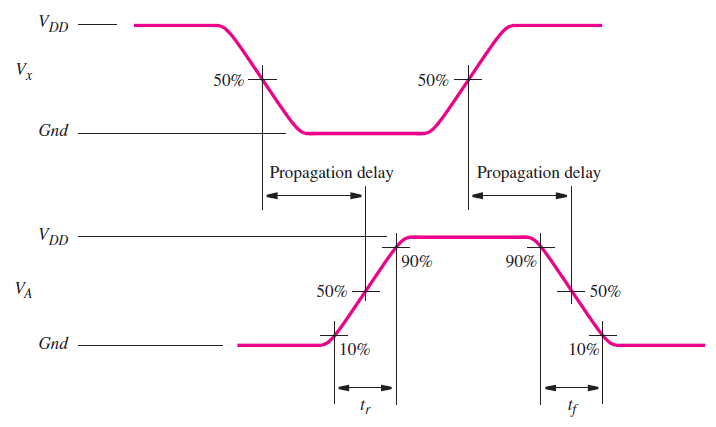
\includegraphics[scale=0.6]{../EJ1/Recursos/time_logic.PNG}
    \caption{Definici\'on te\'orica de los tiempos a medir}
    \label{fig:time_logic}
\end{figure}

\begin{figure}[H]
    \centering
        \begin{tabular}{c c}
            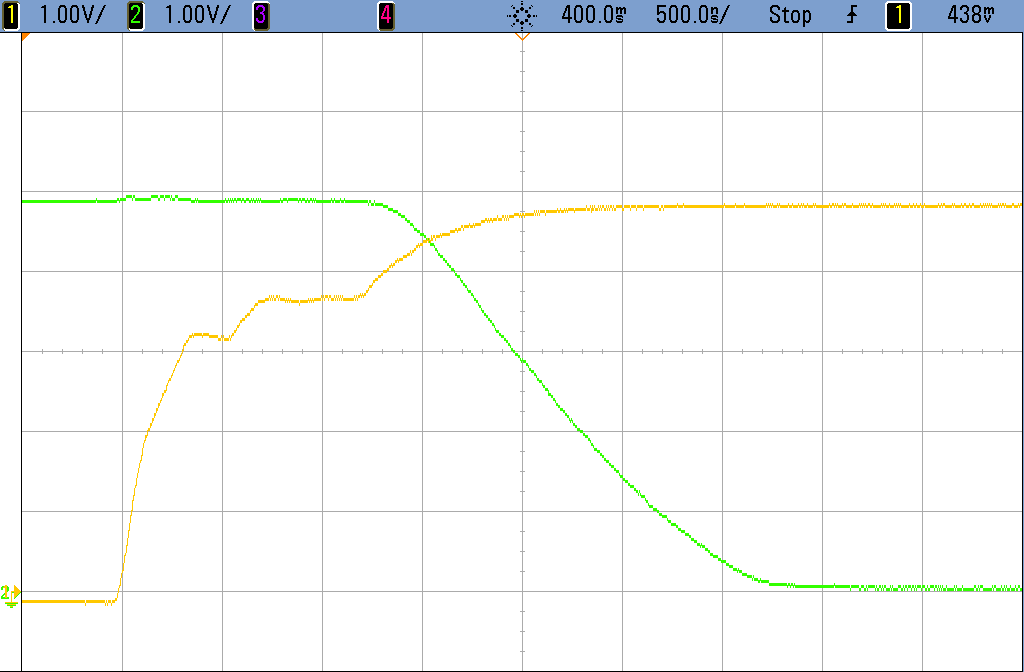
\includegraphics[scale=0.20]{../EJ1/Mediciones/Osciloscopio/Segundo_Intento/Times_RTL/cropped_scope_37.png} &
            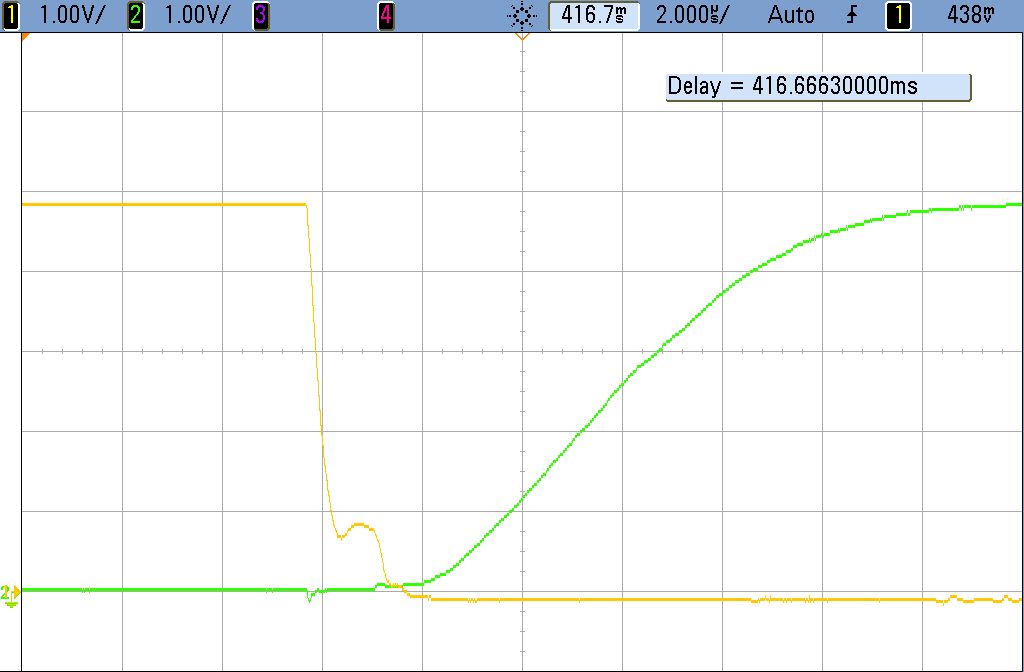
\includegraphics[scale=0.20]{../EJ1/Mediciones/Osciloscopio/Segundo_Intento/Times_RTL/cropped_scope_39.png}
        \end{tabular}
    \caption{Casos ejemplo de medici\'on de los tiempos. Entrada: amarilla, Salida: verde}
    \label{fig:operation_times}
\end{figure}

\begin{table}[H]
    \centering
    \begin{tabular}{c c c c c}
        Circuito & Prop. de alto a bajo & Prop. de bajo a alto & Trans. de alto a bajo & Trans. de bajo a alto \\
        \hline \\
        RTL & $5.49\mu s$ & $1.88\mu s$ & $1.37\mu s$ & $6.12\mu s$ \\
        TTL & $2.81\mu s$ & $55ns$ & $57.2ns$ & $57n s$ \\
        MOS & $15.3\mu s$ & $185ns$ & $177ns$ & $27.4\mu s$ \\
        CMOS & $710ns$ & $720ns$ & $412ns$ & $504ns$ \\
        \hline
    \end{tabular}
    \caption{Medici\'on de los tiempos de operaci\'on sin carga}
\end{table}

\begin{table}[H]
    \centering
    \begin{tabular}{c c c c c}
        Circuito & Prop. de alto a bajo & Prop. de bajo a alto & Trans. de alto a bajo & Trans. de bajo a alto \\
        \hline \\
        RTL & $11.2\mu s$ & $2.75\mu s$ & $2.8\mu s$ & $29.2\mu s$ \\
        TTL & $9.68\mu s$ & $72ns$ & $206ns$ & $27.8 \mu s$ \\
        MOS & $23.4\mu s$ & $210ns$ & $182ns$ & $51.2\mu s$ \\
        CMOS & $750ns$ & $745ns$ & $434ns$ & $532ns$ \\
        \hline
    \end{tabular}
    \caption{Medici\'on de los tiempos de operaci\'on con $C = 1nF$}
\end{table}

\subsubsection{An\'alisis de resultados}
Las cargas capacitivas agregadas a las salidas de las compuertas incrementan los tiempos medidos.
En primer lugar, entre las tecnolog\'ias RTL y TTL, se puede observar una diferencia atribuida a que el mismo transistor empleado en RTL
tiene una etapa previa en TTL que reduce los tiempos con corrientes mayores para los procesos de apagado y encendido de la juntura del transistor de salida.

Por otro lado, al momento de cargar con una determinada capacidad las compuertas, la que menos variaci\'on presenta es la CMOS.

\subsection{Corrientes m\'aximas}
La interconexi\'on de compuertas l\'ogicas requiere un consumo de corriente para lo que es necesario conocer 
las m\'aximas corrientes de estado alto y estado bajo que pueden soportar tales compuertas.

\subsubsection{Proceso de medici\'on}
En la Fig. \ref{fig:maximum_current_process} se ilustra el proceso de medici\'on en el cual se emplea una carga variable para determinar a qu\'e corriente los niveles de tensi\'on
exceden los l\'imites determinados por las secciones anteriores.

\begin{figure}[H]
    \centering
        \begin{tabular}{c c}
            \includegraphics[scale=0.45]{../EJ1/Recursos/maximum_current.png} &
            \includegraphics[scale=0.45]{../EJ1/Recursos/maximum_current_low.png} 
        \end{tabular}
    \caption{Proceso de medici\'on de m\'axima corriente}
    \label{fig:maximum_current_process}
\end{figure}

\begin{table}[H]
    \centering
    \begin{tabular}{c c c}
        Circuito & IOH & IOL \\
        \hline \\
        RTL & $14.4 \mu A$ & $488\mu A$ \\
        TTL & $14.6 \mu A$ & $13.1 \mu A$ \\
        MOS & $11.5 \mu A$ & $249 \mu A$ \\
        CMOS & $15.2mA$ & $135\mu A$ \\
        \hline
    \end{tabular}
    \caption{Mediciones de corriente m\'axima sin carga}
\end{table}

\begin{table}[H]
    \centering
    \begin{tabular}{c c c}
        Circuito & IOH & IOL \\
        \hline \\
        RTL & $11.1 \mu A$ & $1.13m A$ \\
        TTL & $10.2 \mu A$ & $49.5 \mu A$ \\
        MOS & $12.4 \mu A$ & $37.7 \mu A$ \\
        CMOS & $21.3mA$ & $102\mu A$ \\
        \hline
    \end{tabular}
    \caption{Mediciones de corriente m\'axima con carga $C = 1nF$}
\end{table}

\subsubsection{An\'alisis de resultados}
Las compuertas RTL, TTL, MOS tienen una corriente similar de IOH por la resistencia de pull-up de aproximadamente $R = 10k \Omega$. 

A pesar de esto \'ultimo, cada una de tales tecnolog\'ias difiere de las dem\'as en la corriente IOL justamente porque est\'a definida por el control de la condici\'on de saturaci\'on en los BJT, y la zona \'ohmica en el caso
Las peque\~nas diferencias se dan por los procesos de transici\'on entre estados de los dispositivos empleados, sean BJT o MOSFET. 
No obstante, dado que en el circuito CMOS los MOSFETS son complementarios, no se encontr\'o razonamiento por el cual la corriente IOH sea tan diferente con respecto de IOL, se asume que es por las condiciones
en las que pudieran encontrarse los modelos usados.

\subsection{Dise\~no de PCB}

\begin{figure}[H]
    \centering
        \begin{tabular}{c c}
            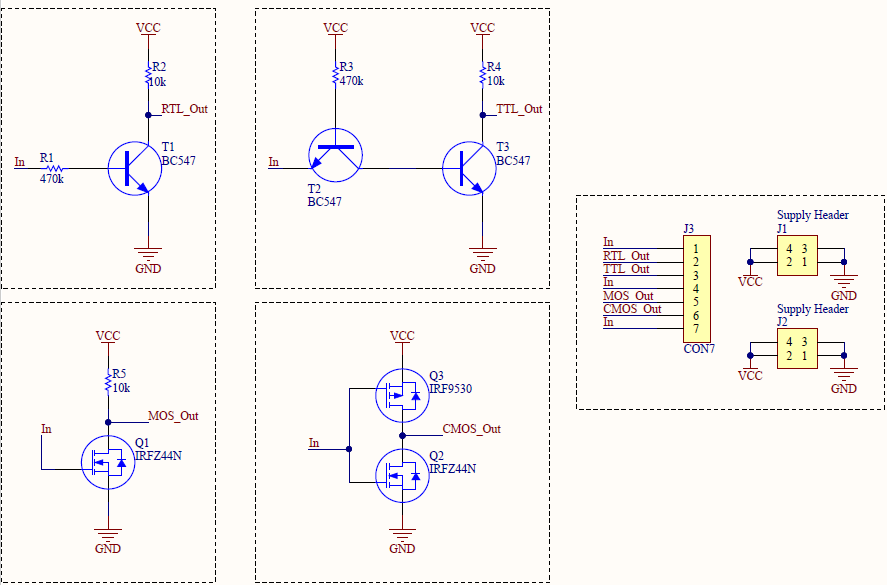
\includegraphics[scale=0.4]{../EJ1/Recursos/esquematico.PNG} &
            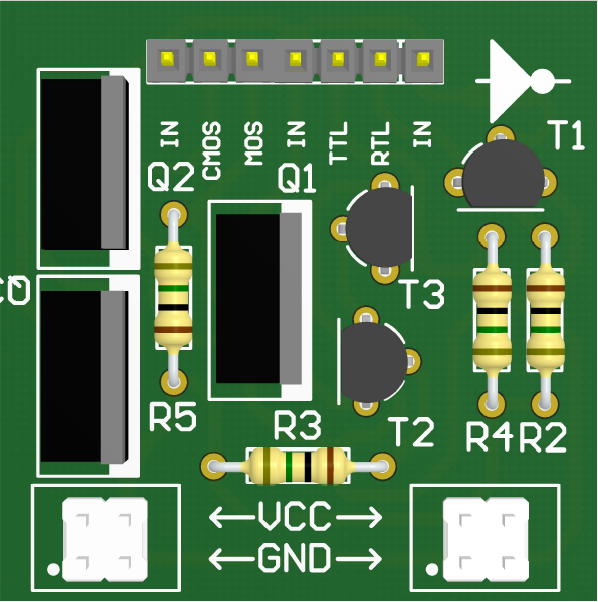
\includegraphics[scale=0.3]{../EJ1/Recursos/pcb3d.PNG} 
        \end{tabular}
    \caption{Dise\~no del PCB en Altium Designer}
    \label{fig:pcb_design_nots}
\end{figure}

\subsection{Observaciones}

\subsubsection{Resistencia de pull-down}
En la Fig. \ref{fig:pull_down_error} se observa la salida de la compuerta RTL con entrada al aire con y sin resistencia de pull-down en la entrada. Puede observarse que al no quedar bien definido el estado,
la salida no est\'a bien definida seg\'un las mediciones obtenidas de los niveles de tensi\'on.

\begin{figure}[H]
    \centering
    \begin{tabular}{c c}
        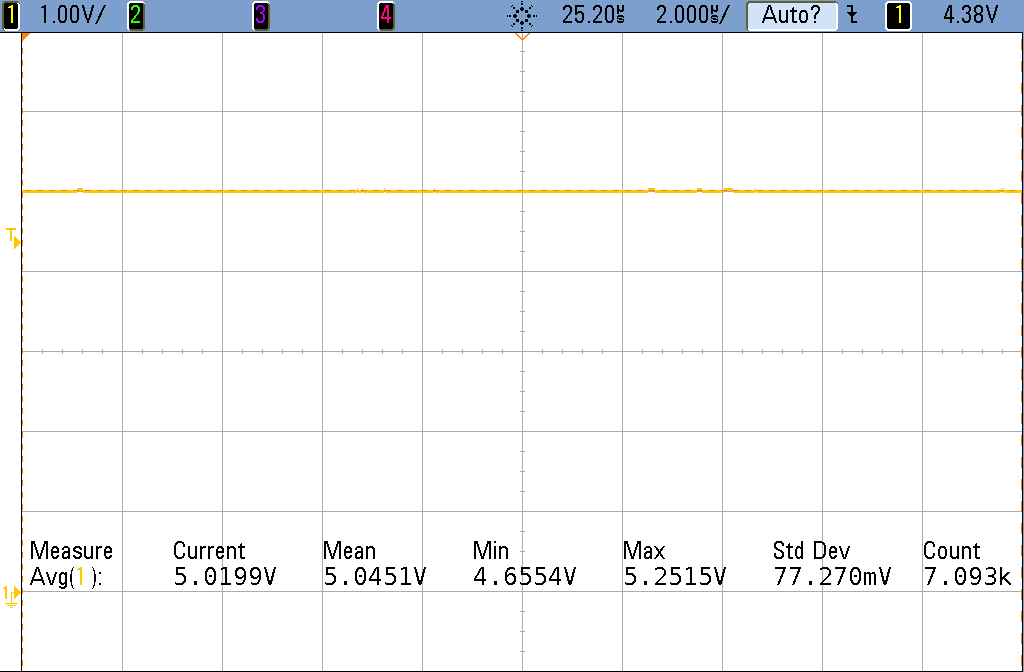
\includegraphics[scale=0.2]{../EJ1/Mediciones/Osciloscopio/Observaciones/Pull_down_error/cropped_scope_14.png} & 
        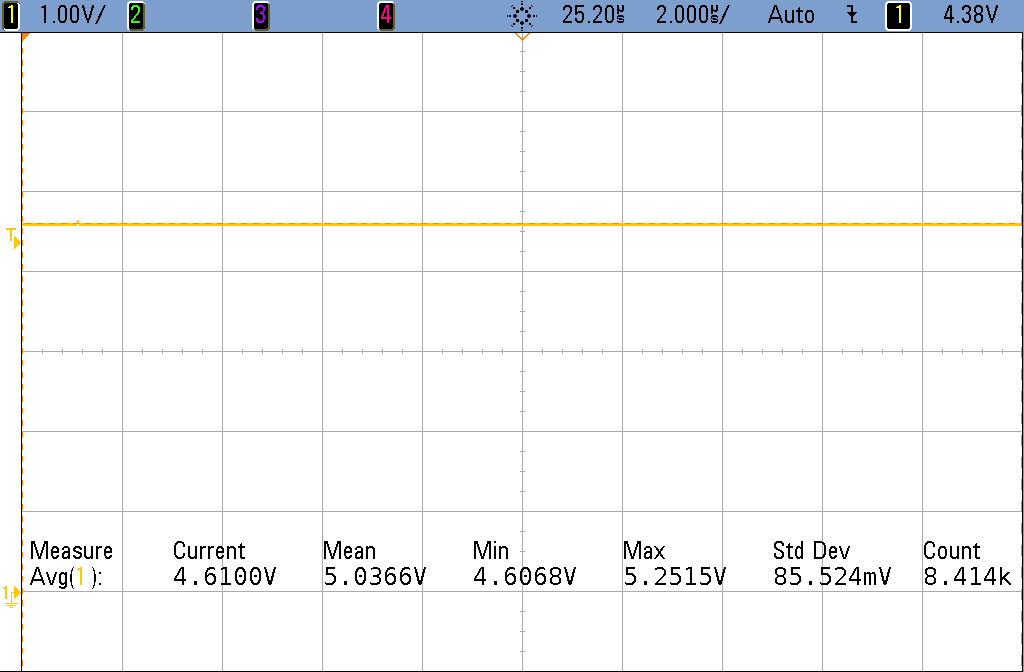
\includegraphics[scale=0.2]{../EJ1/Mediciones/Osciloscopio/Observaciones/Pull_down_error/cropped_scope_15.png}
    \end{tabular}
    \caption{Medici\'on de la salida de un RTL con entrada al aire}
    \label{fig:pull_down_error}
\end{figure}

\subsubsection{Tiempos de transici\'on}
En la Fig. \ref{fig:rtl_fixed} se ilustran los tiempos de transici\'on de la salida de una compuerta RTL modificando la resistencia de base del transistor.
Puede observarse que a pesar de que diversas resistencias son posibles para alcanzar las condiciones de saturaci\'on y corte, no todas producen la misma corriente de encendido y apagado,
con lo cual esto puede producir que diferentes alternativas sean m\'as r\'apidas que otras, a expensas de un mayor consumo de corriente. El circuito no tiene capacitor de desacople, esto permite
observar que en el caso de mayor corriente y menor tiempo, se producen mayores distorsiones en la se\~nal de entrada.

\begin{figure}[H]
    \centering
        \begin{tabular}{c c}
            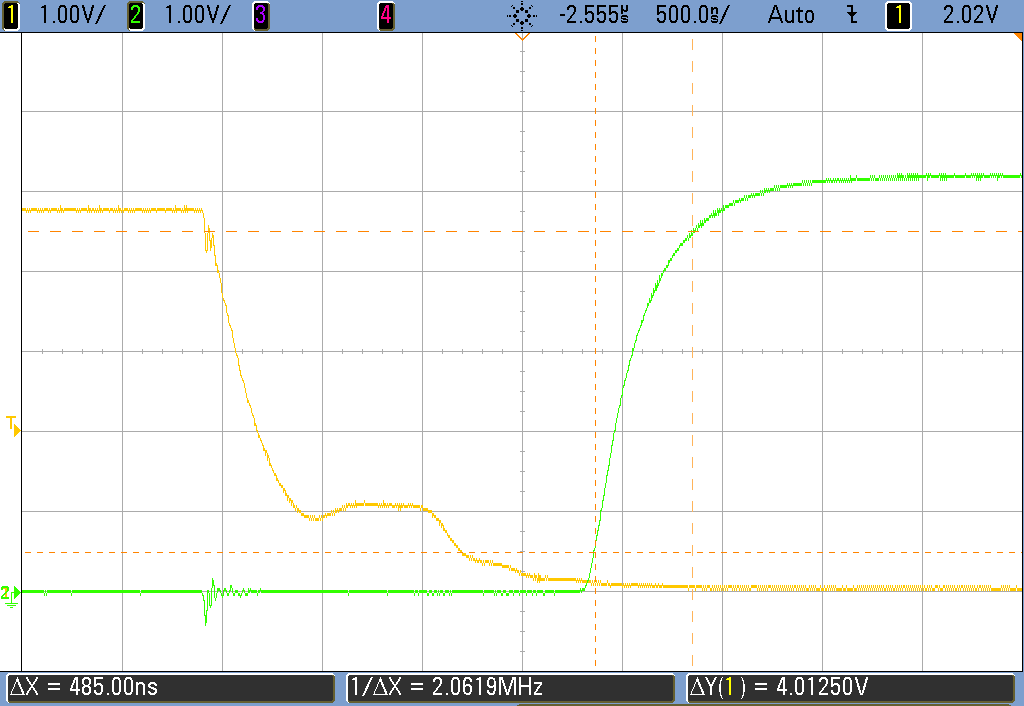
\includegraphics[scale=0.2]{../EJ1/Mediciones/Osciloscopio/Observaciones/Mejora_polarizacion_RTL/cropped_scope_20.png} &
            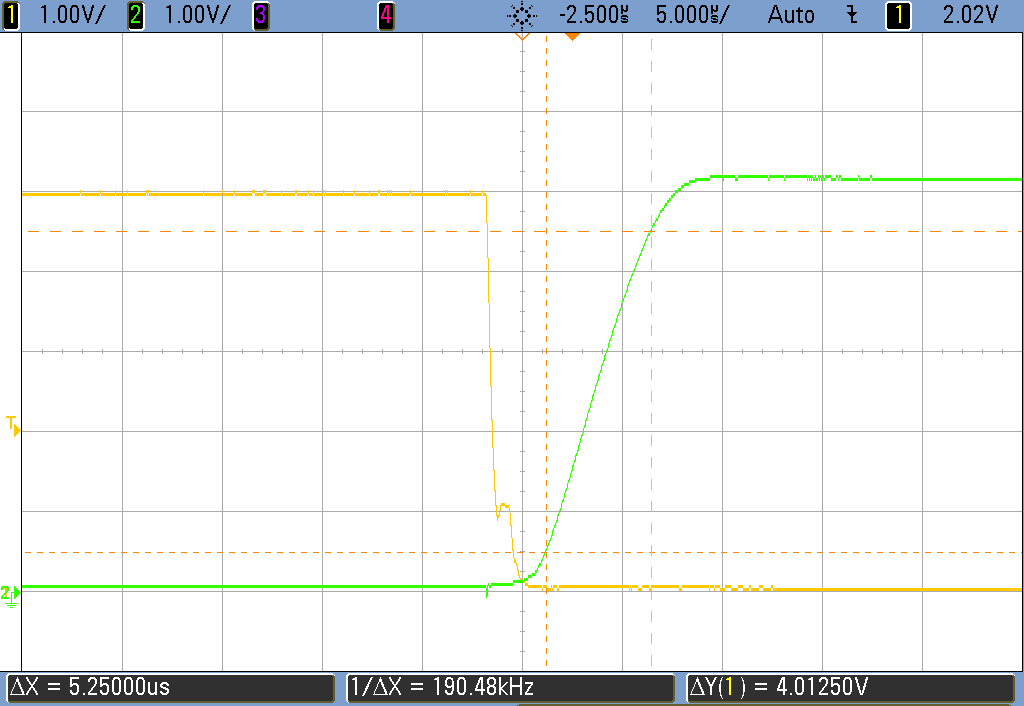
\includegraphics[scale=0.2]{../EJ1/Mediciones/Osciloscopio/Observaciones/Mejora_polarizacion_RTL/cropped_scope_21.png}
        \end{tabular}
    \caption{Medici\'on de tiempo de transici\'on en RTL. Entrada: amarilla, Salida: verde}
    \label{fig:rtl_fixed}
\end{figure}

\subsubsection{Mediciones}
En la Fig. \ref{fig:mos_problem_signal} se puede observar que en la transici\'on de la compuerta MOS se produjeron algunas distorsiones en las se\~nales de entrada y de salida.
Luego de analizar diferentes puntos de vista, se concluy\'o que el problema inicial est\'a dado por el hecho de que las cuatro compuertas l\'ogicas implementadas est\'an funcionando
en forma simult\'anea y conectadas en paralelo a la salida, lo cual provoca que en las mediciones de la MOS se introduzcan perturbaciones del transitorio de los BJT. Adem\'as, el funcionamiento
conjunto en las transiciones implica un consumo de corriente que en un intervalo de tiempo peque\~no produce una ca\'ida de tensi\'on que pudo ser corregida con capacitores de desacople.

\begin{figure}[H]
    \centering
        \begin{tabular}{c c}
            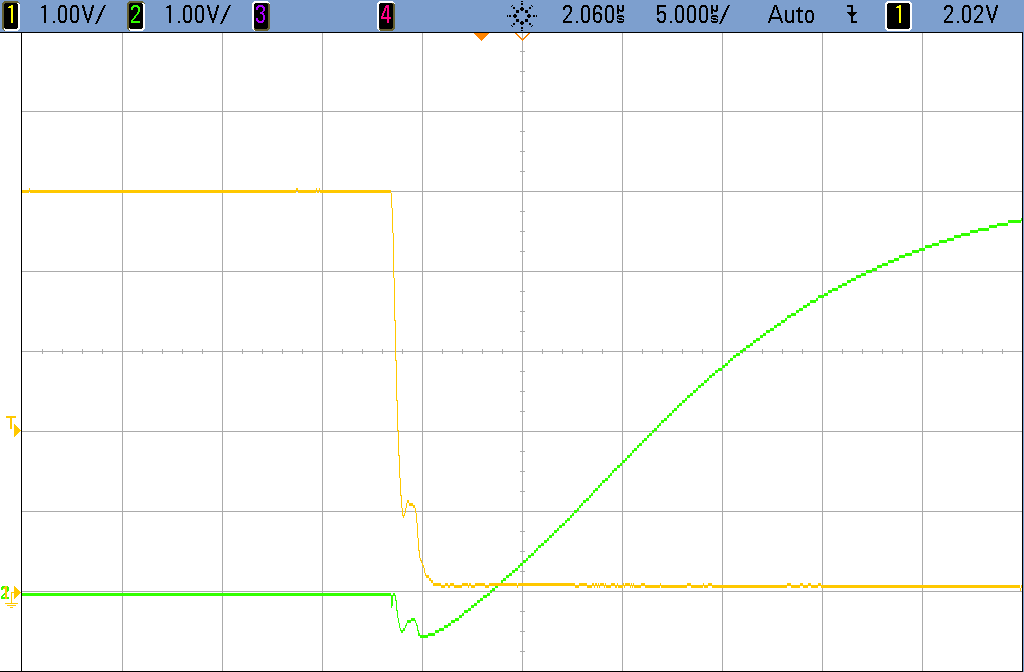
\includegraphics[scale=0.2]{../EJ1/Mediciones/Osciloscopio/Observaciones/Mejora_transicion_MOS/cropped_scope_14.png} &
            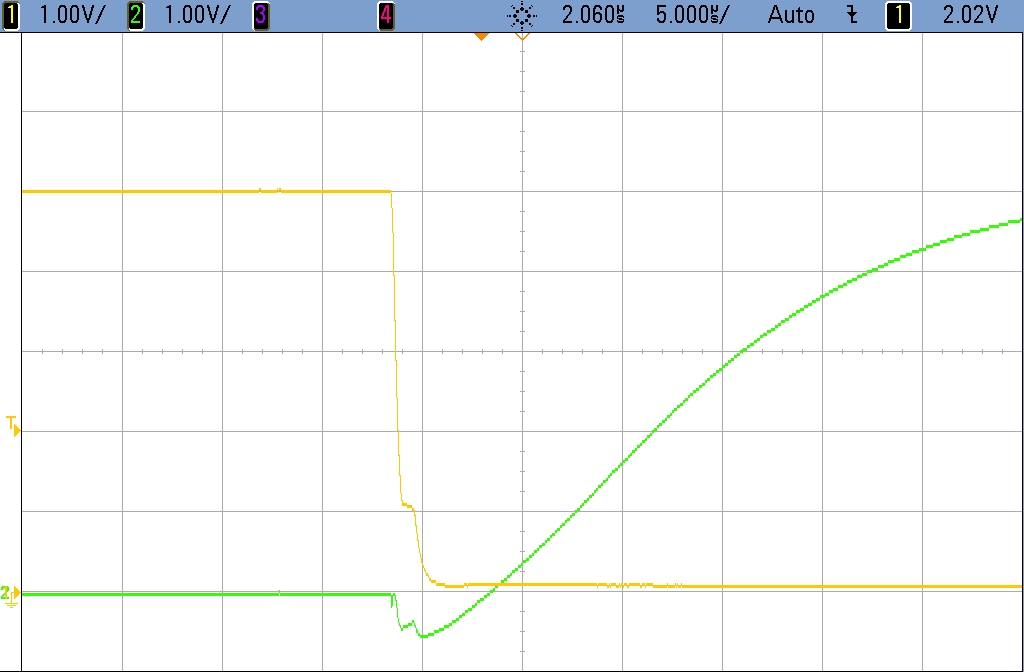
\includegraphics[scale=0.2]{../EJ1/Mediciones/Osciloscopio/Observaciones/Mejora_transicion_MOS/cropped_scope_15.png} 
        \end{tabular}
    \caption{Transici\'on de estados en la compuerta MOS. Entrada: amarilla, Salida: verde}
    \label{fig:mos_problem_signal}
\end{figure}

\subsection{Conclusiones}
En t\'erminos generales todas las compuertas implementadas presentan estados l\'ogicas de salida bien definidos, no obstante destaca por sus m\'argenes de ruido uniformes la compuerta MOS.
Luego, comparando los tiempos de operaci\'on, sin carga la de mayor velocidad es la TTL, aunque se puede observar que la MOS y la CMOS son las que logran mantener mejor sus caracter\'isticas
frente a las cargas capacitivas, esto implica que la velocidad superior de la TTL se mantiene seg\'un la carga, no obstante las propiedades de una MOS se mantiene con peque\~nas variaciones. Finalmente, en este aspecto,
RTL queda claramente en desventaja frente a las dem\'as, difiriendo en varios \'ordenes de magnitud.
Por \'ultimo, sin considerar la corriente IOH del caso CMOS, se puede concluir que las compuertas MOS y CMOS tuvieron una mayor capacidad de entregar corriente,
en parte resulta razonable considerando que pose\'ian un mayor margen de ruido.

En conclusi\'on, en diversos aspectos las compuertas CMOS y MOS destacan por sus caracter\'isticas. Las compuertas TTL tienen una mejor performance en t\'erminos de velocidad seg\'un la carga.
Es importante mencionar que las caracter\'isticas temporales de las compuertas pudieron haber sido mejoradas incrementando los consumos de corrientes al reducir las resistencias que las controlan.